%%%%%%%%%%%%%%%%%%%%%%%%%%%%%%%%%%%%%%%%%
% Short Sectioned Assignment
% LaTeX Template
% Version 1.0 (5/5/12)
%
% This template has been downloaded from:
% http://www.LaTeXTemplates.com
%
% Original author:
% Frits Wenneker (http://www.howtotex.com)
%
% License:
% CC BY-NC-SA 3.0 (http://creativecommons.org/licenses/by-nc-sa/3.0/)
%
%%%%%%%%%%%%%%%%%%%%%%%%%%%%%%%%%%%%%%%%%

%----------------------------------------------------------------------------------------
%	PACKAGES AND OTHER DOCUMENT CONFIGURATIONS
%----------------------------------------------------------------------------------------

\documentclass[paper=a4, fontsize=11pt]{scrartcl} % A4 paper and 11pt font size

\usepackage[T1]{fontenc} % Use 8-bit encoding that has 256 glyphs
%\usepackage{fourier} % Use the Adobe Utopia font for the document - comment this line to return to the LaTeX default
\usepackage[english]{babel} % English language/hyphenation
\usepackage{amsmath,amsfonts,amsthm} % Math packages

\usepackage{lipsum} % Used for inserting dummy 'Lorem ipsum' text into the template

\usepackage{graphicx}
\usepackage{caption}
\usepackage{subcaption}

\usepackage{sectsty} % Allows customizing section commands
\allsectionsfont{\centering \normalfont\scshape} % Make all sections centered, the default font and small caps

\usepackage{fancyhdr} % Custom headers and footers
\pagestyle{fancyplain} % Makes all pages in the document conform to the custom headers and footers
\fancyhead{} % No page header - if you want one, create it in the same way as the footers below
\fancyfoot[L]{} % Empty left footer
\fancyfoot[C]{} % Empty center footer
\fancyfoot[R]{\thepage} % Page numbering for right footer
\renewcommand{\headrulewidth}{0pt} % Remove header underlines
\renewcommand{\footrulewidth}{0pt} % Remove footer underlines
\setlength{\headheight}{13.6pt} % Customize the height of the header

\numberwithin{equation}{section} % Number equations within sections (i.e. 1.1, 1.2, 2.1, 2.2 instead of 1, 2, 3, 4)
\numberwithin{figure}{section} % Number figures within sections (i.e. 1.1, 1.2, 2.1, 2.2 instead of 1, 2, 3, 4)
\numberwithin{table}{section} % Number tables within sections (i.e. 1.1, 1.2, 2.1, 2.2 instead of 1, 2, 3, 4)

\setlength\parindent{0pt} % Removes all indentation from paragraphs - comment this line for an assignment with lots of text

%----------------------------------------------------------------------------------------
%	TITLE SECTION
%----------------------------------------------------------------------------------------

\newcommand{\horrule}[1]{\rule{\linewidth}{#1}} % Create horizontal rule command with 1 argument of height

\title{	
\normalfont \normalsize 
\textsc{ETH Zurich, D-INFK} \\ [25pt] % Your university, school and/or department name(s)
\horrule{0.5pt} \\[0.4cm] % Thin top horizontal rule
\huge Computer Vision: Exercise 4 \\ % The assignment title
\horrule{2pt} \\[0.5cm] % Thick bottom horizontal rule
}

\author{Igor Pesic} % Your name

\date{\normalsize\today} % Today's date or a custom date

\begin{document}

\maketitle % Print the title


\section{Line Fitting with RANSAC}

In Figure \ref{fig:ransacLine} are shown the fitted lines for the given points. The black line represents the real model, the green is the one fitted with the least squares and and the red one is fitted with RANSAC. As we can see, RANSAC has performed very well, and also much better than least squares. This is because RANSAC only fits the model based on the inliers and thus is very robust to the outliers in comparison to the least squares. Error with RANSAC (with 73 inliers) was 691.2084 and with least squares was 681.0276. Lower error of least squares algorithm is expected since that is the objective that is directly minimized.

\begin{figure}[h!]
\centering
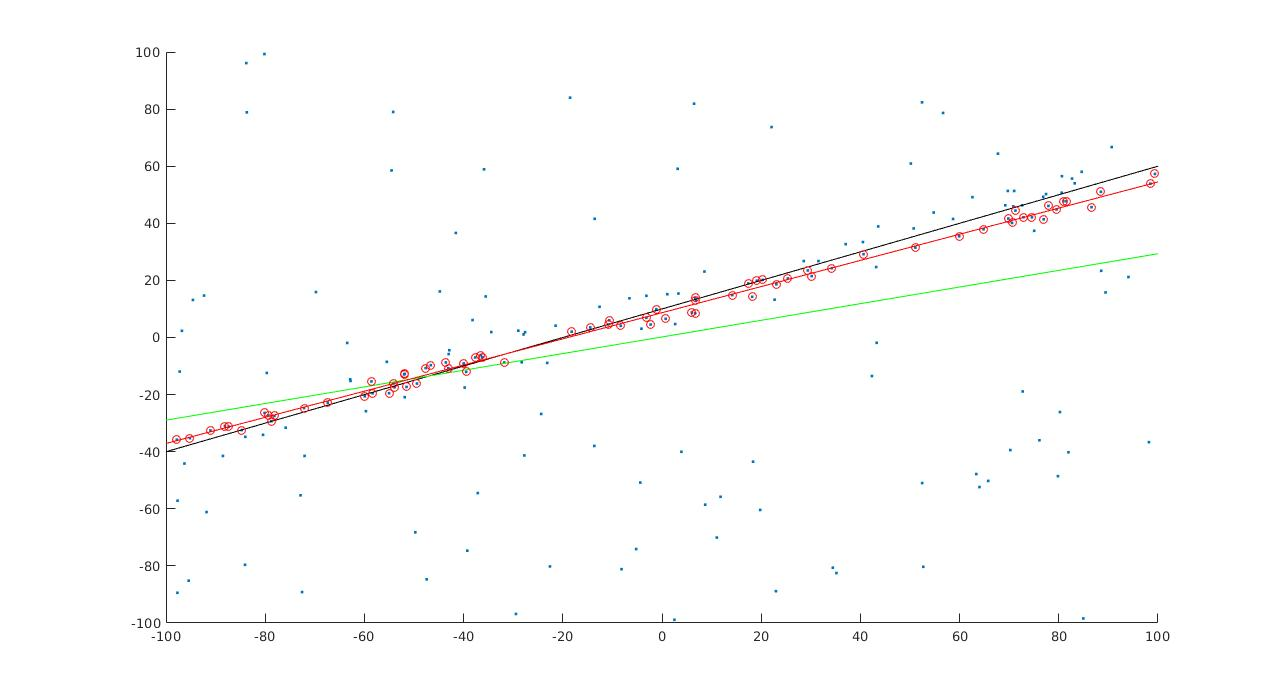
\includegraphics[width=0.7\textwidth]{ransacLine.jpg}
\caption{Line fitted with LS and RANSAC.}
\label{fig:ransacLine}
\end{figure}


\section{Fundamental Matrix}

The Figures \ref{fig:f} and \ref{fig:fh} show the epipolar lines obtained by both unconstrained and constrained fundamental matrix. In both cases the points were normalized and the fundamental matrix was denormalized.
\begin{figure}
\centering
\begin{subfigure}{.5\textwidth}
  \centering
  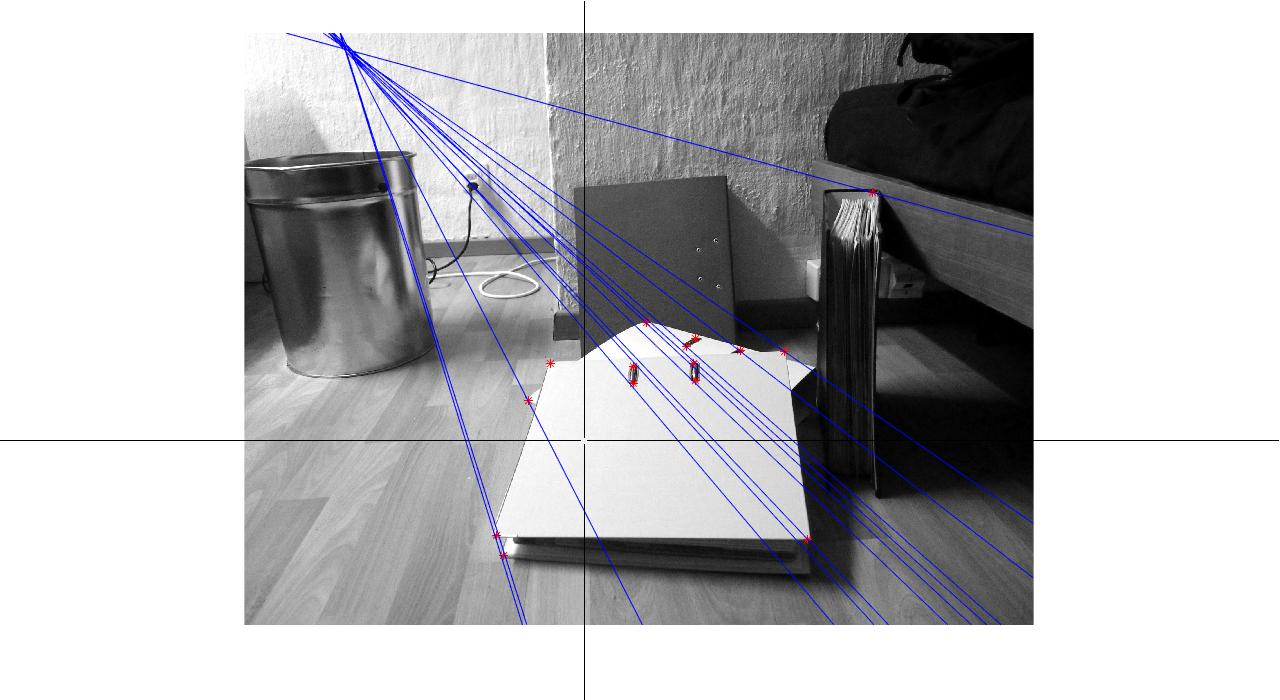
\includegraphics[width=1.5\linewidth]{f1.jpg}
  \caption{Left}
\end{subfigure}%
\begin{subfigure}{.7\textwidth}
  \centering
  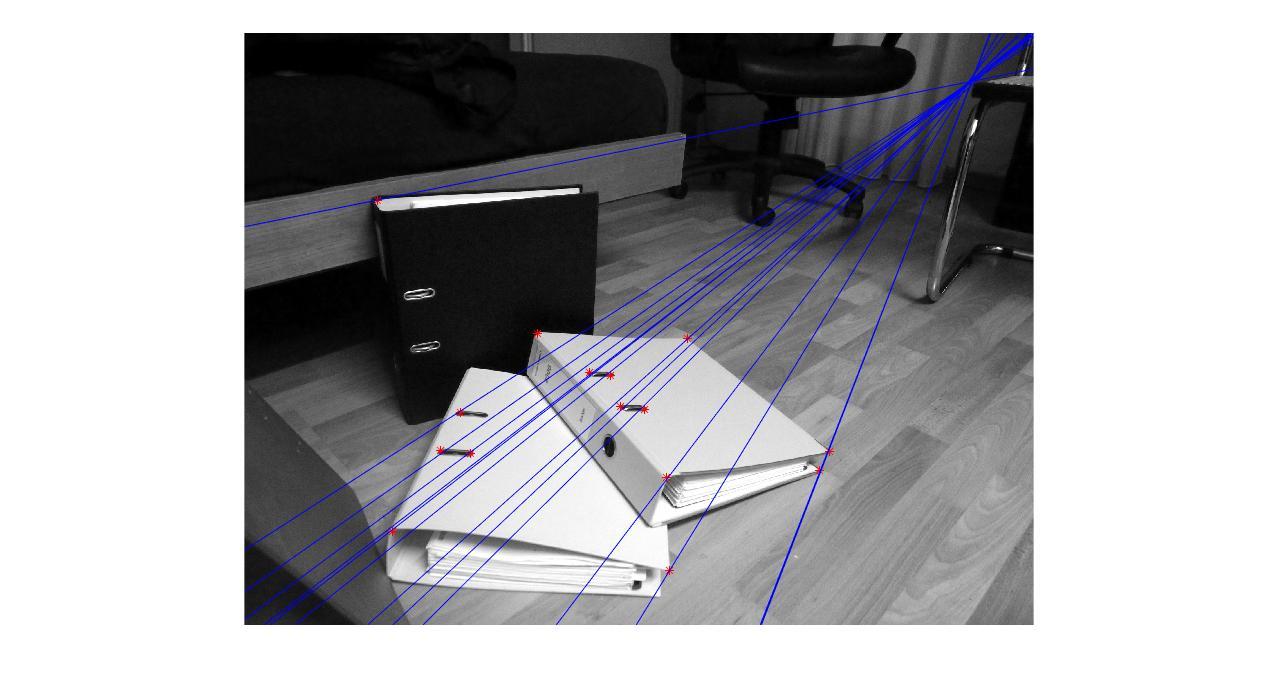
\includegraphics[width=1.1\linewidth]{f2.jpg}
  \caption{Right}
\end{subfigure}
\caption{Obtained with Unconstrained Fundamental Matrix}
\label{fig:f}
\end{figure}

\begin{figure}
\centering
\begin{subfigure}{.5\textwidth}
  \centering
  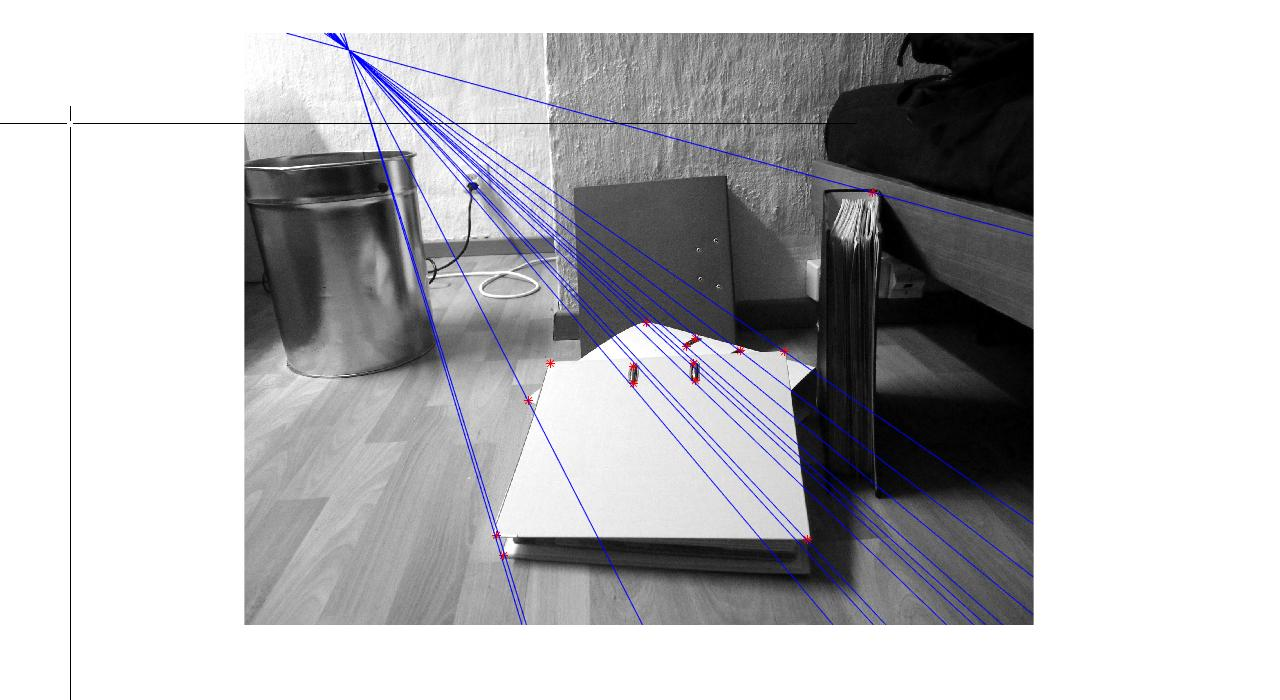
\includegraphics[width=1.5\linewidth]{fh1.jpg}
  \caption{Left}
\end{subfigure}%
\begin{subfigure}{.7\textwidth}
  \centering
  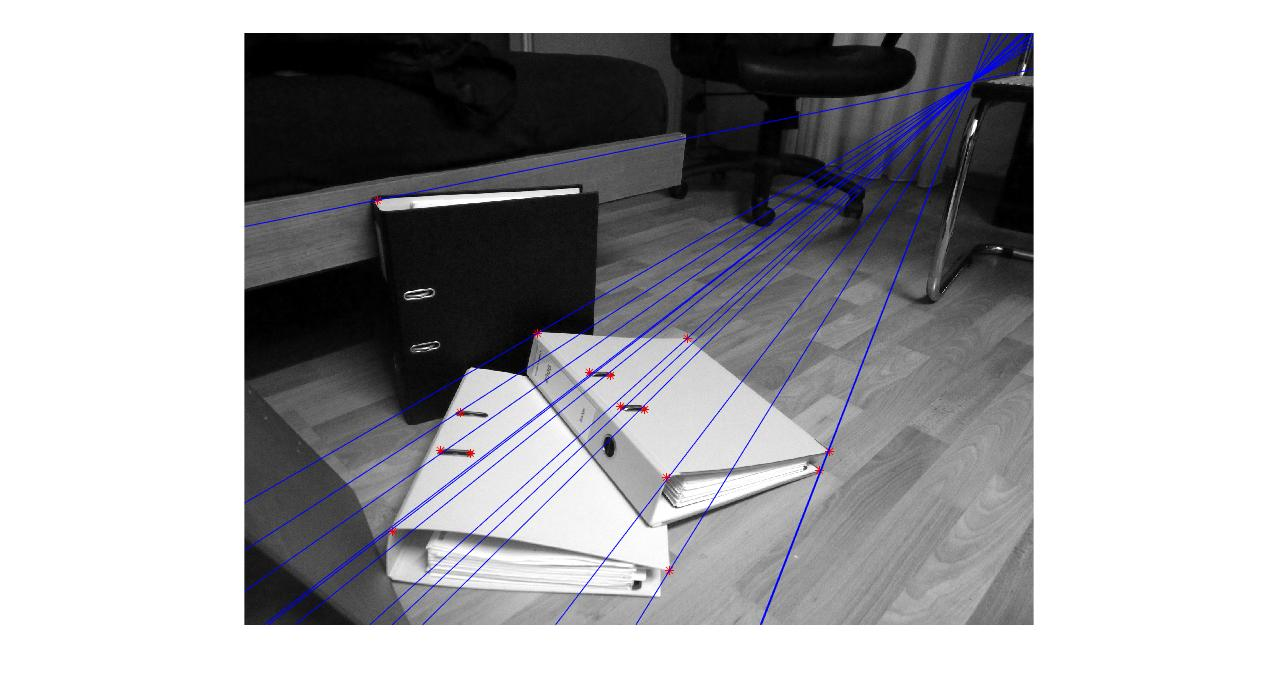
\includegraphics[width=1.1\linewidth]{fh2.jpg}
  \caption{Right}
\end{subfigure}
\caption{Obtained with Constrained Fundamental Matrix}
\label{fig:fh}
\end{figure}


\section{Essential Matrix}
Same as in the previous section, here I also present epipolar lines (figures \ref{fig:e} and \ref{fig:eh}) from both unconstrained and constrained Fundamental matrix, but this time the lines are obtained by normalizing the points with camera calibration matrix K and then denormalizing the obtained essential matrix E to fundamental matrix F.\\
The following are the obtained (constrained) matrices (F is from the previous section):
\[ E=
\begin{bmatrix}
-0.123043889725867	& 5.95442555256993	& 2.39708269015134 \\
7.58535258787966 &	-0.562008696217138	& 3.04984669403554 \\
2.81965957105025 &	-3.35900913477464 &	-0.162594823748377
\end{bmatrix}
\]
\[ K^{-T}  E  K^{-1}=
\begin{bmatrix}
-4.5004e-08 & 	2.1754e-06 &	-8.4179e-05 \\
2.7713e-06 &	-2.0511e-07 &	-0.0007 \\
-0.00026	& -0.0040	& 0.2474
\end{bmatrix}
\]
\[ F=
\begin{bmatrix}
-1.37288e-07 &	2.3807e-06	& -6.8534e-05 \\
2.5125e-06	& 1.4240e-07 &	-0.0007 \\
-5.7192e-05	& -0.00444 &	0.2117
\end{bmatrix}
\]
 
\begin{figure}
\centering
\begin{subfigure}{.5\textwidth}
  \centering
  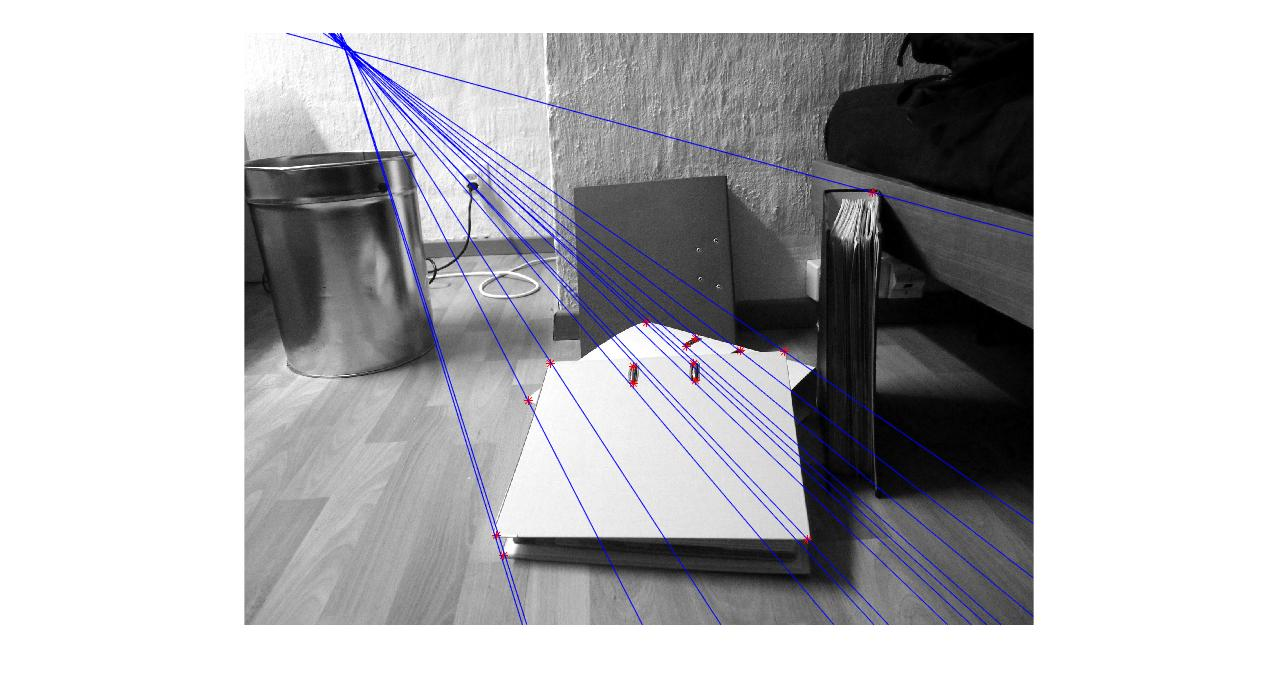
\includegraphics[width=1.5\linewidth]{e1.jpg}
  \caption{Left}
\end{subfigure}%
\begin{subfigure}{.7\textwidth}
  \centering
  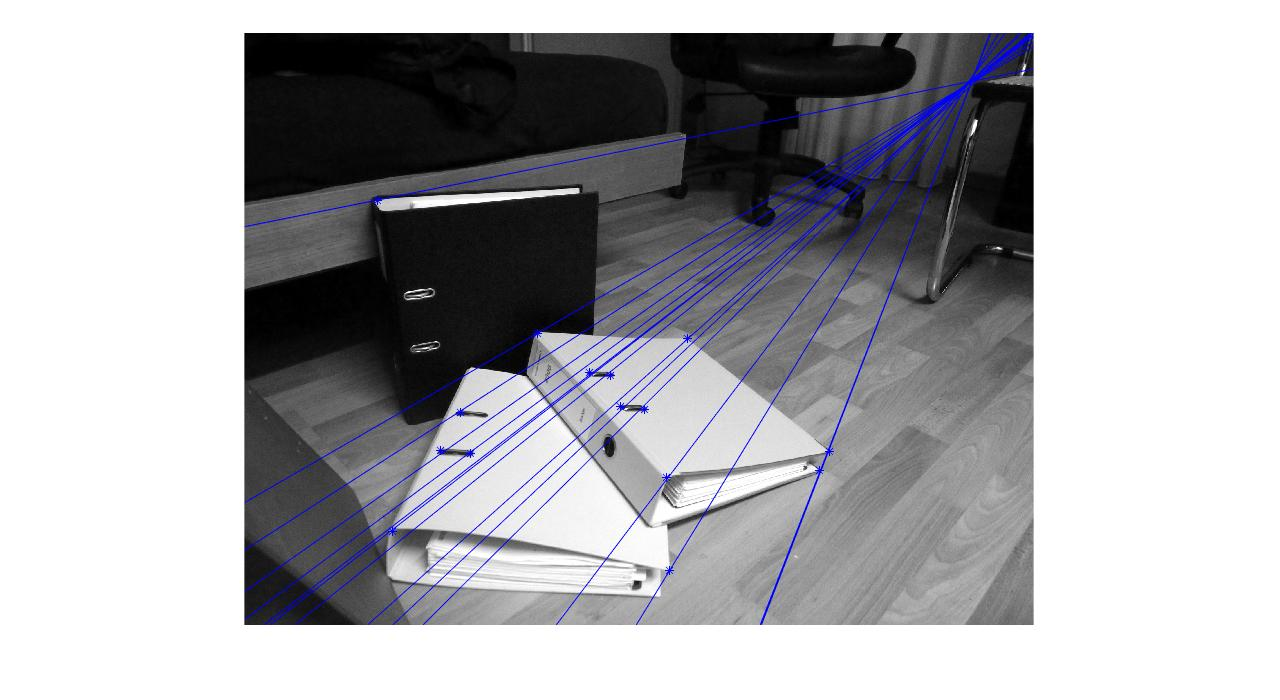
\includegraphics[width=1.1\linewidth]{e2.jpg}
  \caption{Right}
\end{subfigure}
\caption{Obtained with Unconstrained Essential Matrix}
\label{fig:f}
\end{figure}

\begin{figure}
\centering
\begin{subfigure}{.5\textwidth}
  \centering
  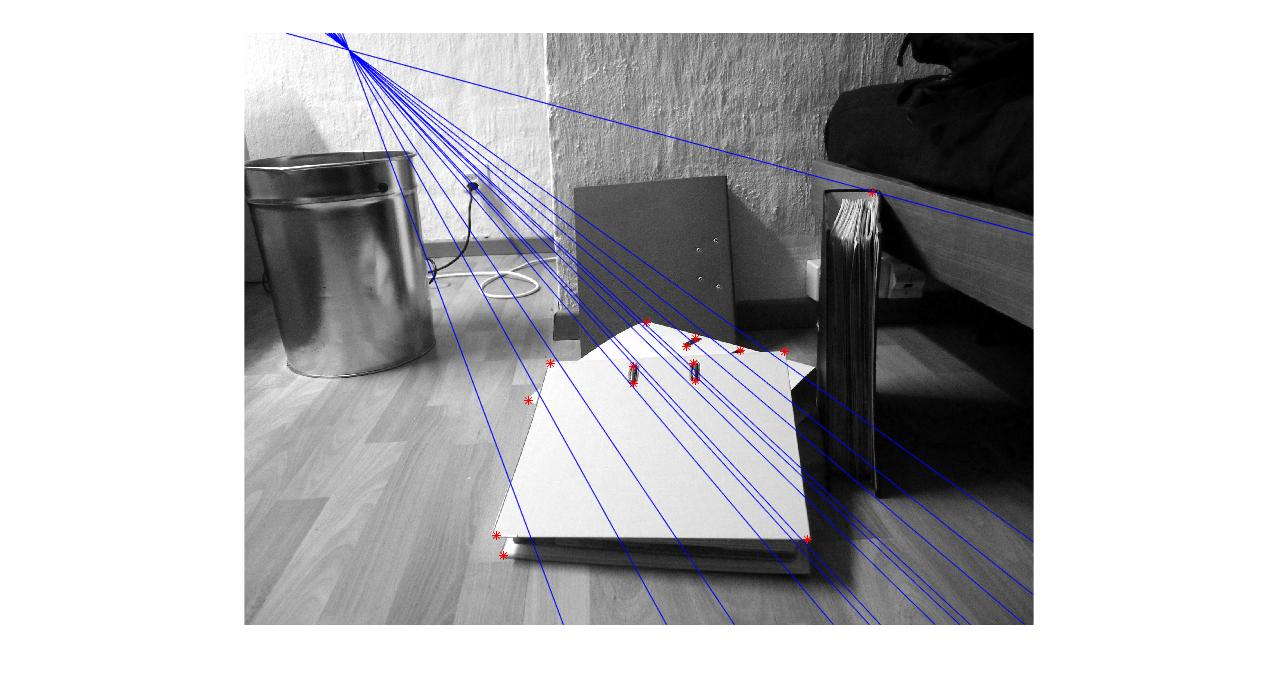
\includegraphics[width=1.5\linewidth]{eh1.jpg}
  \caption{Left}
\end{subfigure}%
\begin{subfigure}{.7\textwidth}
  \centering
  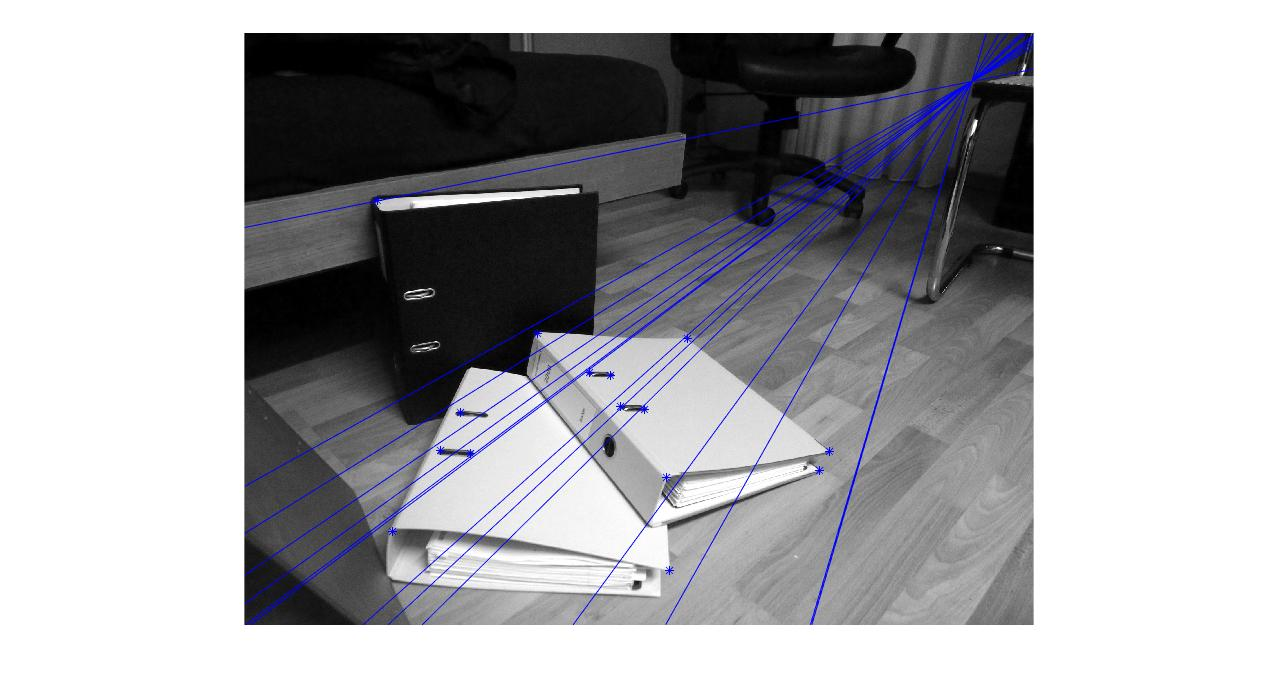
\includegraphics[width=1.1\linewidth]{eh2.jpg}
  \caption{Right}
\end{subfigure}
\caption{Obtained with Constrained Essential Matrix}
\label{fig:fh}
\end{figure}

\section{Decomposition of Essential Matrix}
I have decomposed E as following: $R_1 = U * W * V^T$ and $R_2 = U * W^T * V^T$, $t=U(:,end)$ with W is as described in exercise slides. Then $P_1=[R_1|t]$, $P_2=[R_1|-t]$, $P_3=[R_2|t]$, $P_4=[R_2|-t]$. By using the triangulation and making sure that all $X$ and $PX$ have positive $z$ coordinate I have chosen $P_1$. Figure \ref{fig:camera} plots the camera (3D).

\begin{figure}[h!]
\centering
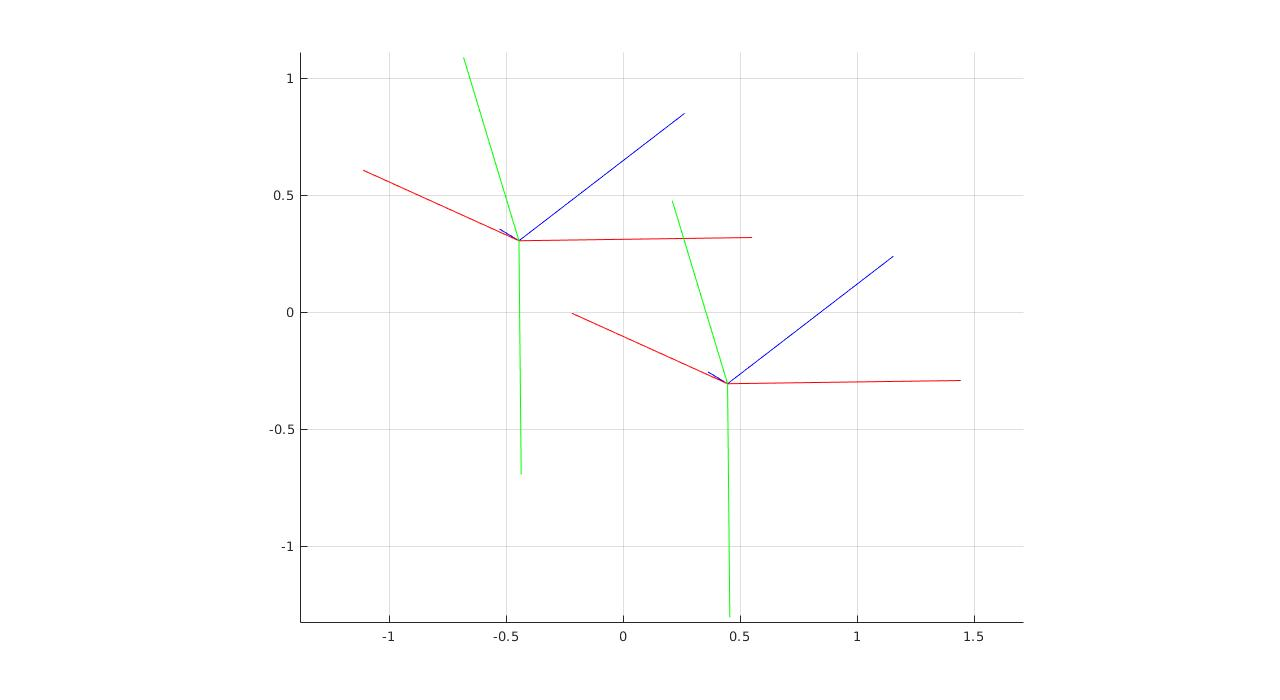
\includegraphics[width=0.7\textwidth]{cameras.jpg}
\caption{Camera plot.}
\label{fig:camera}
\end{figure}		

\section{Feature extraction and matching}		

The Figure \ref{fig:sift} shows the matched features in the image pair. Since there is a rotation between the cameras it is expected that not all the lines between the matches are parallel.

\begin{figure}[h!]
\centering
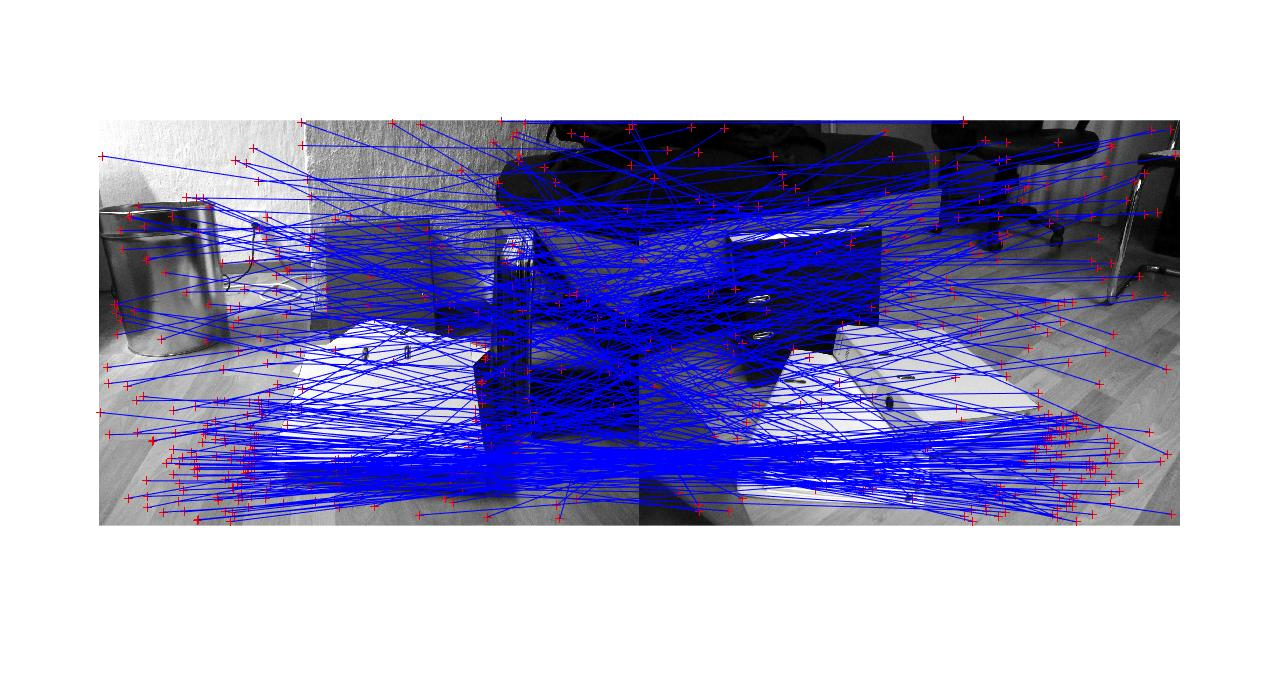
\includegraphics[width=1.2\textwidth]{sift.jpg}
\caption{SIFT: matched features.}
\label{fig:sift}
\end{figure}

\section{8-Point RANSAC}
I tried to implement it with Sampson distance, but it did not work. Somehow all the distances were very large, in the order of $10^5$.

\end{document}